% !TEX root = ../main.tex

\section{PCB Layout and Assembly}
\label{sec:pcb}

\scaffold{
  \textbf{Paragraph 1, layout.} Describe \cref{fig:pcb-layout}: a two-layer board with 149 footprints, the four jacks along one edge, the jack blocks repeated four times, the power section with one copper fill per rail and the regulators between them. Ground is poured on both layers; the power input section has its own pour on the same net. 15 test points sit on the signals the measurements of \cref{ch:results} need: the shift-register lines (TP1--TP4), SPI0 with both chip selects and ready lines (TP5--TP11) and the four rails (TP12--TP15).
}

\begin{figure}[htbp]
  \centering
  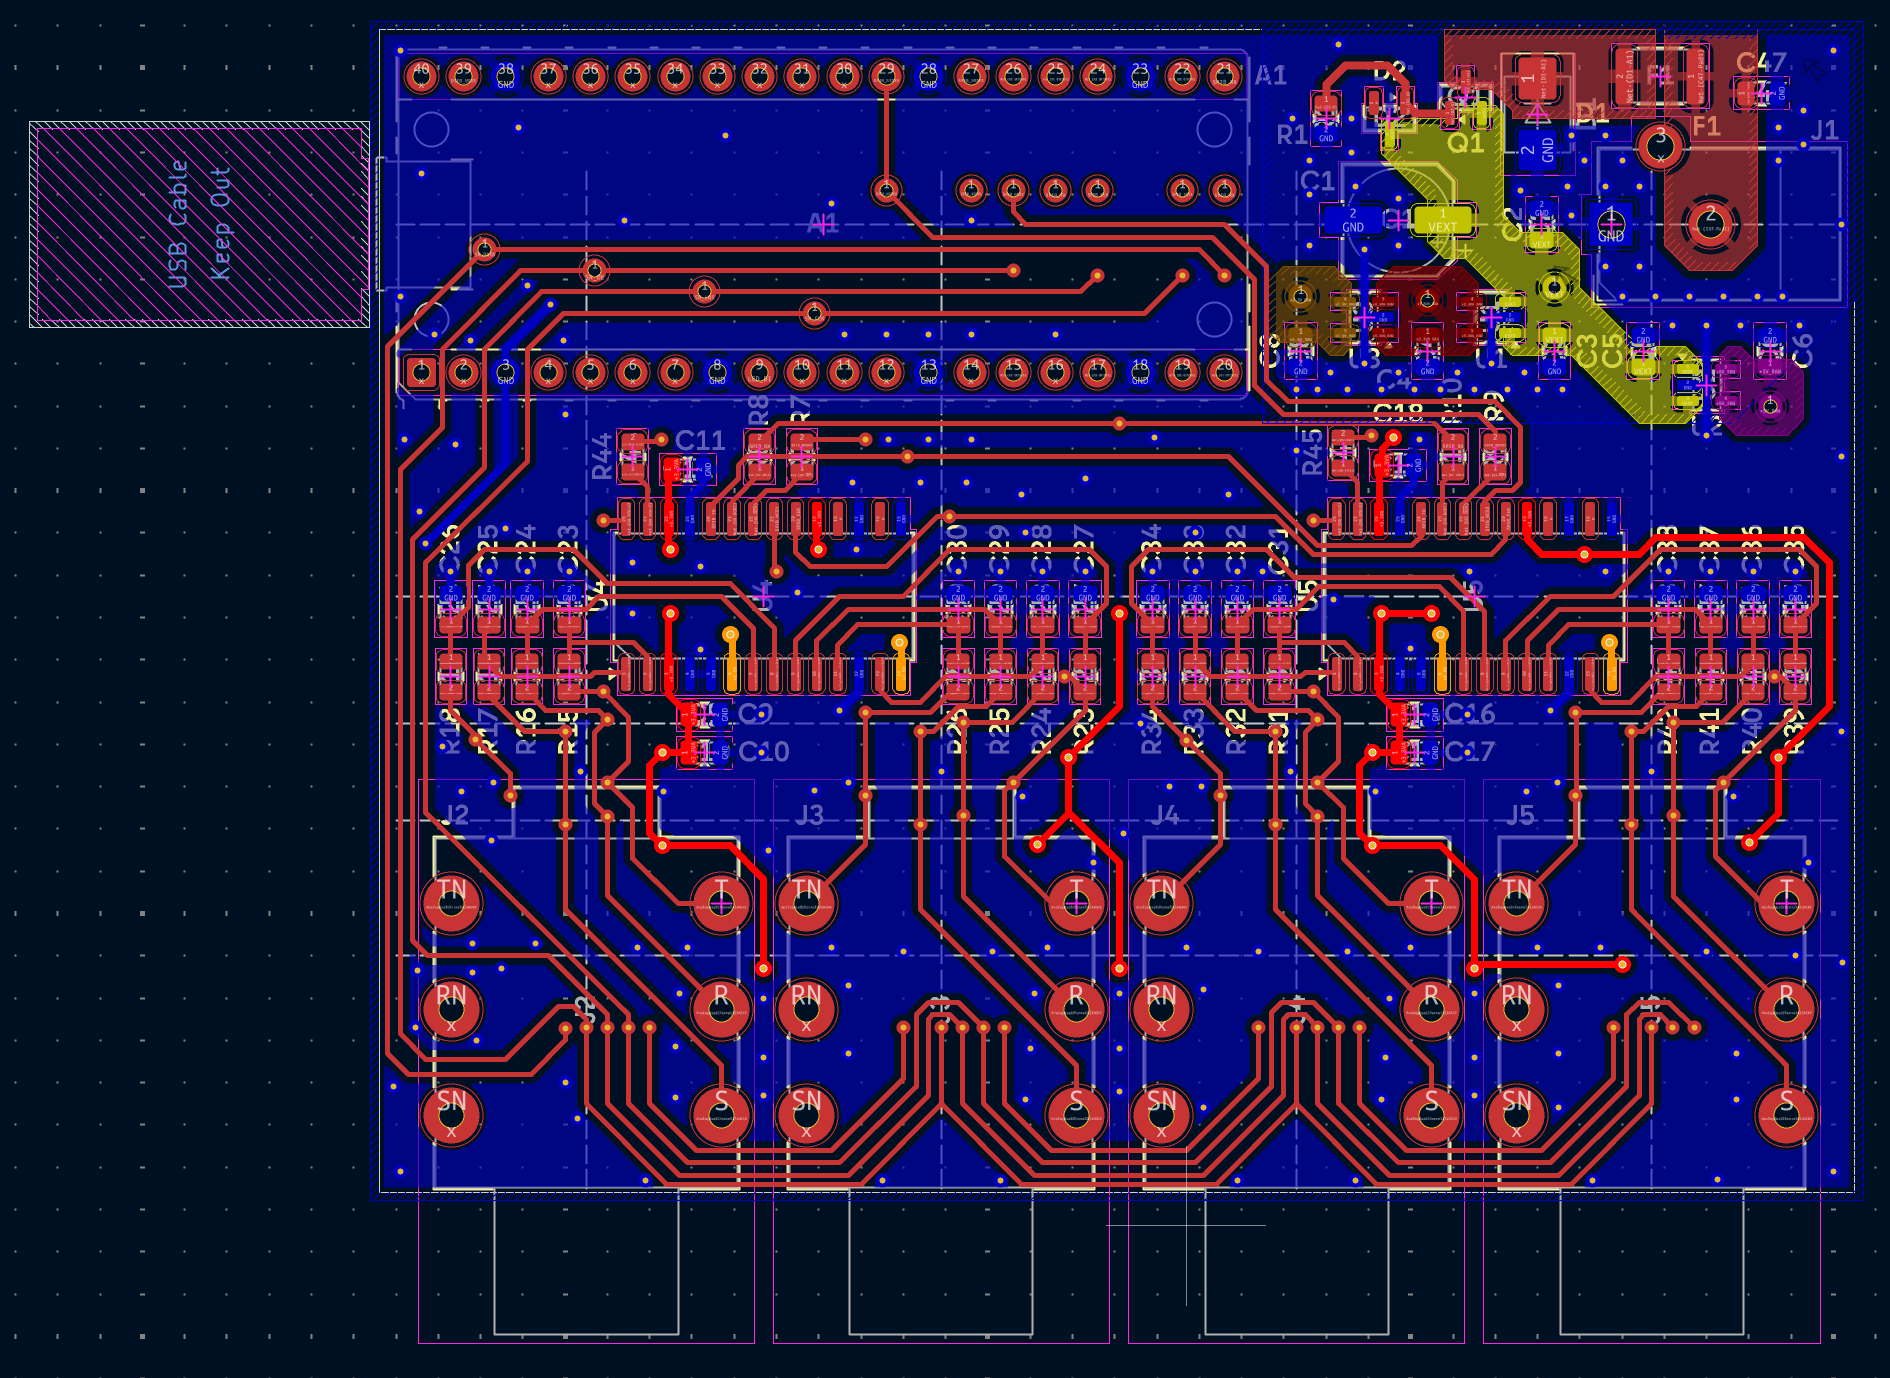
\includegraphics[width=0.85\linewidth]{04-implementation/figures/pcb-layout}
  \titledcaption{PCB Layout}{\scaffoldinline{Name the regions (jacks, four channel blocks, ADCs, microcontroller, power section) and the two copper layers shown. Source: KiCad \code{hardware/ExpressionController.kicad\_pcb}.}}
  \label{fig:pcb-layout}
\end{figure}

\scaffold{
  \textbf{Paragraph 2, assembly.} The top side was soldered by hand in separate blocks, the power supply first, and every rail was checked before the next block was populated; the bottom side was assembled with a stencil (first use for the author). The TMUX1511 in TSSOP-14 were the most difficult parts. Show \cref{fig:assembly}. The board-level self-test passed on its first run (\cref{sec:results-self-test}).
}

\begin{figure}[htbp]
  \centering
  \begin{subfigure}[t]{0.32\linewidth}
    \centering
    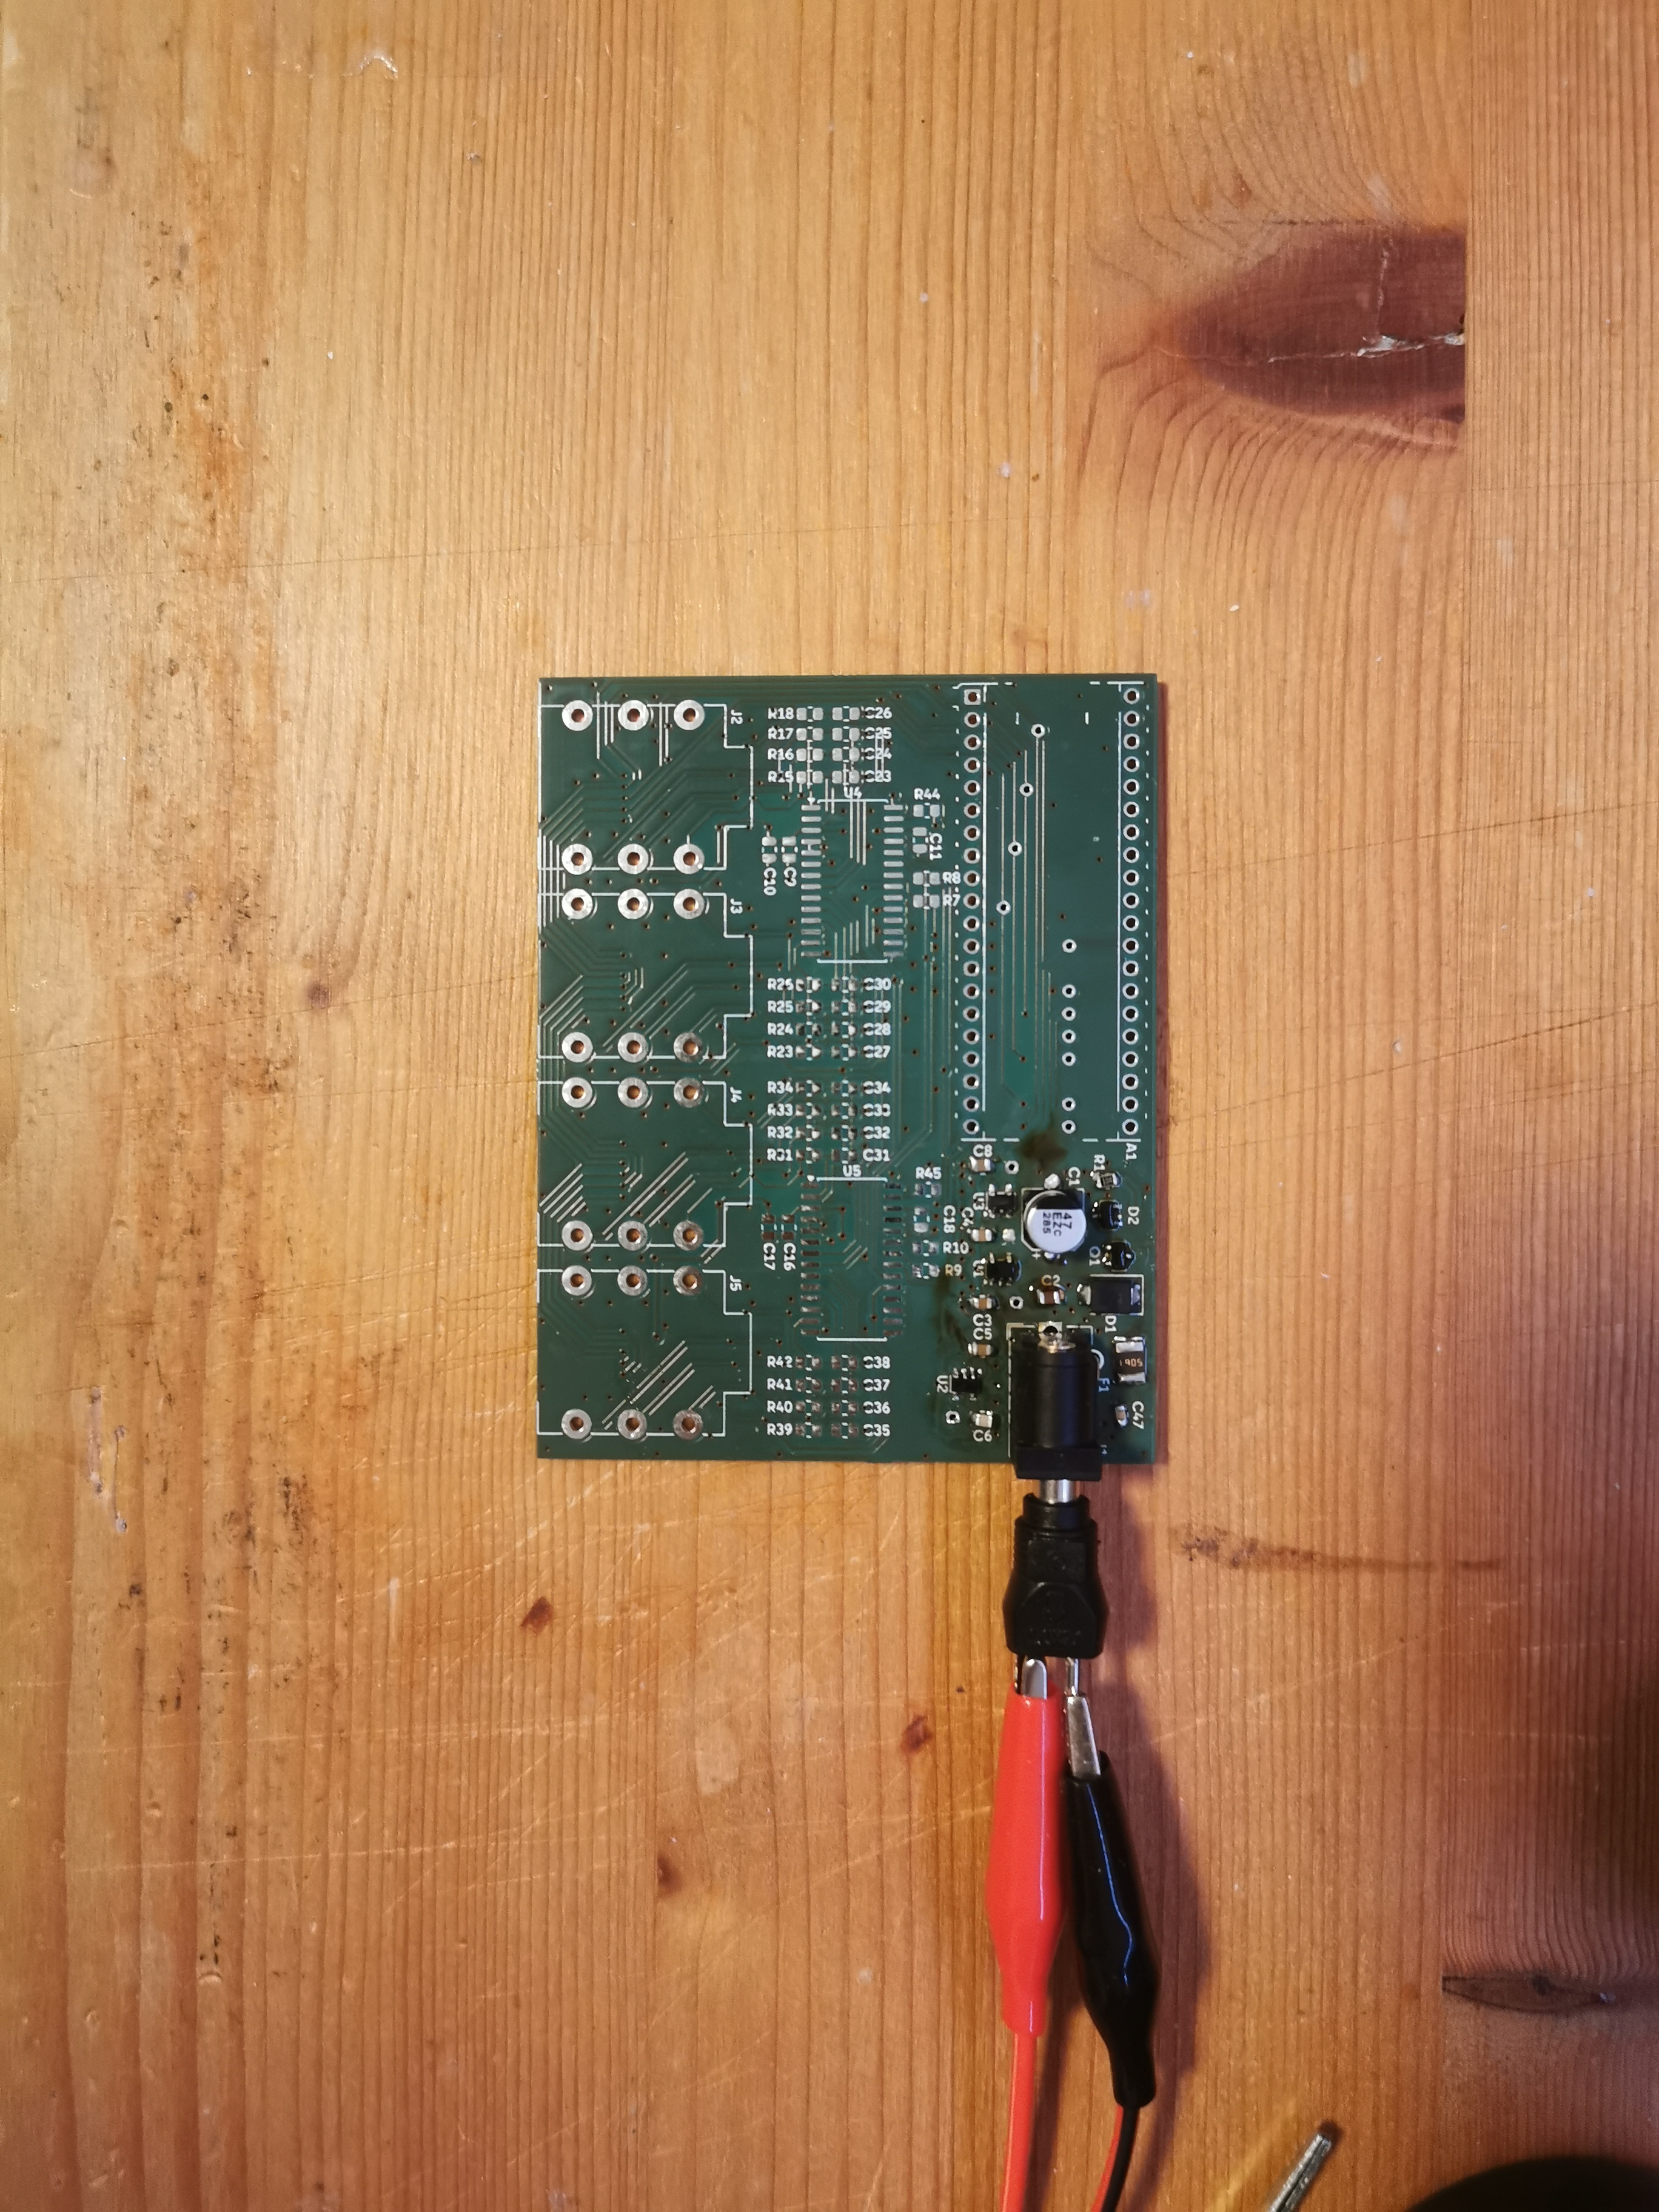
\includegraphics[width=\linewidth]{04-implementation/figures/assembly-top-side}
    \caption{Power Supply Populated}
    \label{fig:assembly-top-side}
  \end{subfigure}%
  \hfill%
  \begin{subfigure}[t]{0.64\linewidth}
    \centering
    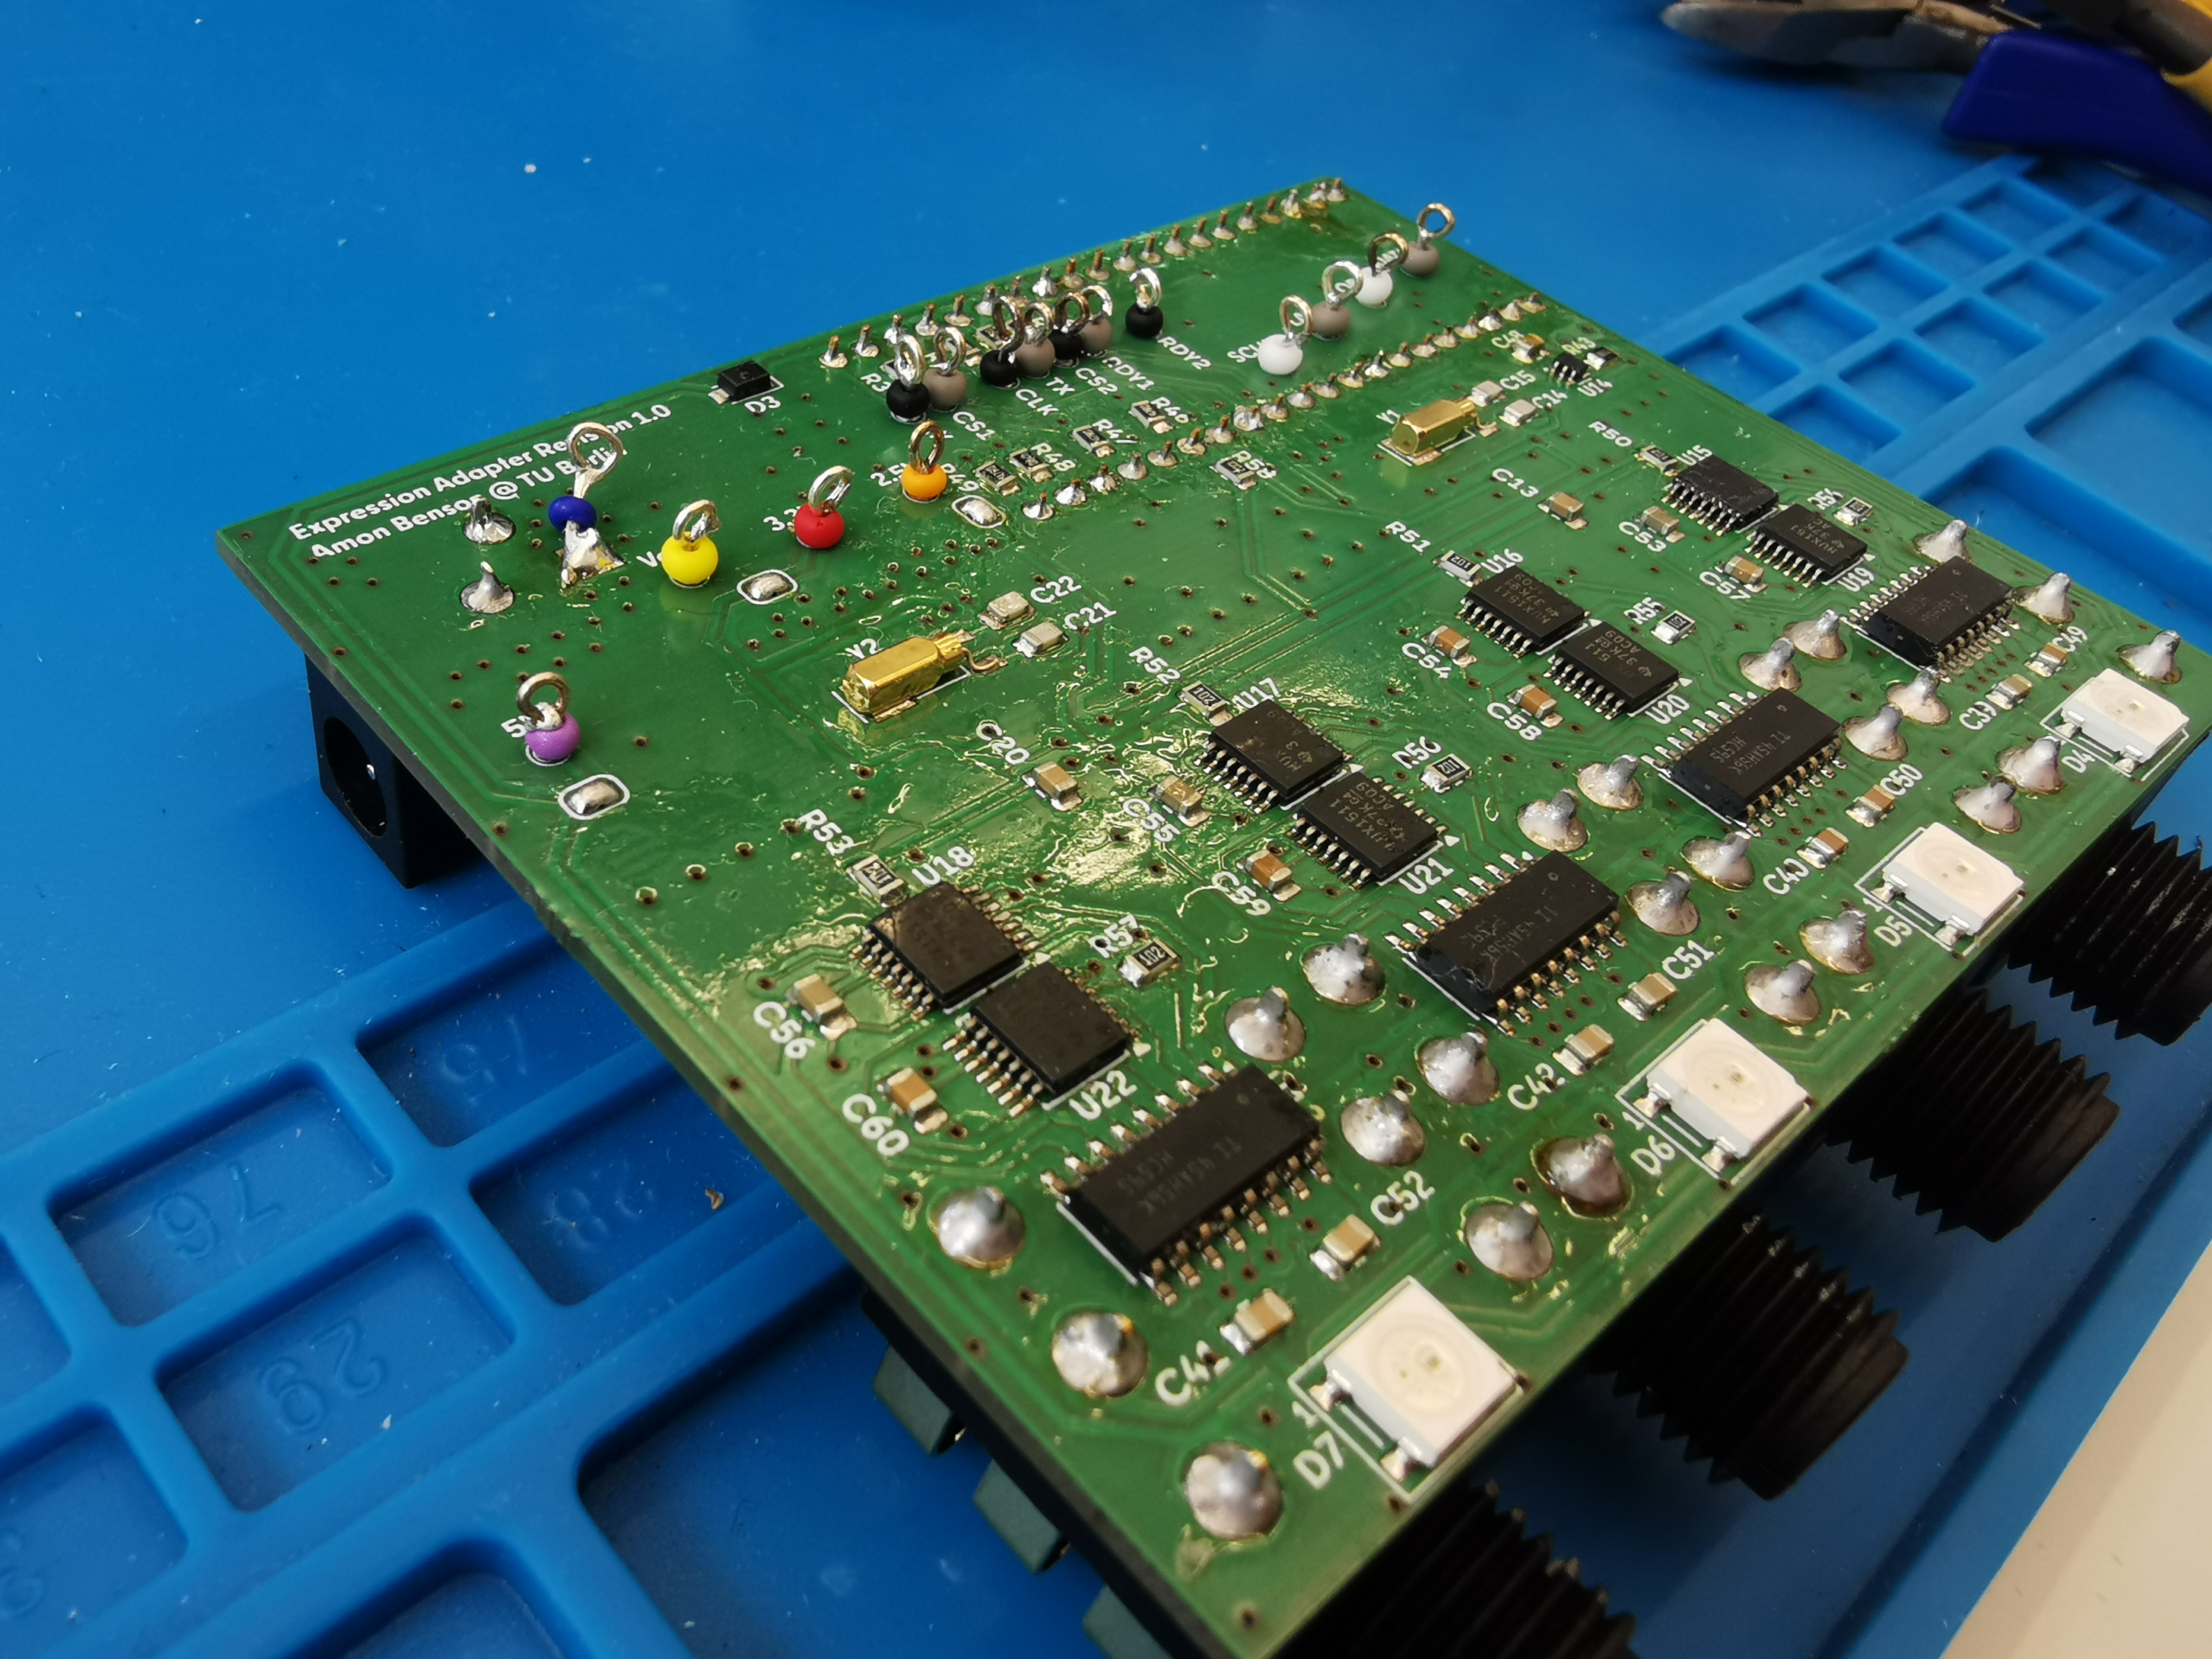
\includegraphics[width=\linewidth]{04-implementation/figures/assembly-complete}
    \caption{Assembled Board}
    \label{fig:assembly-complete}
  \end{subfigure}
  \titledcaption{PCB Assembly}{\scaffoldinline{(a) first assembly stage, check what is populated; (b) the assembled board with the switches, shift registers, ADCs and color-coded test points. Photos of the author; further photos in the folder \enquote{Final Images}.}}
  \label{fig:assembly}
\end{figure}

\openquestion{Board facts}{
  Give the board outline (about \qtyproduct{89 x 70}{\milli\metre} from the ground pour, not measured), the manufacturer of PCB and stencil, and the date the boards were ordered and arrived (git history: final assembly files 6~September, \enquote{after final fab order} 16~September, first firmware on the board 25~September~2026).
}
